\subsection{Complex alignments}\label{GLOBALsec:limitations}

\begin{figure}[t]
  \centering
  \subfloat[High error rate]
    {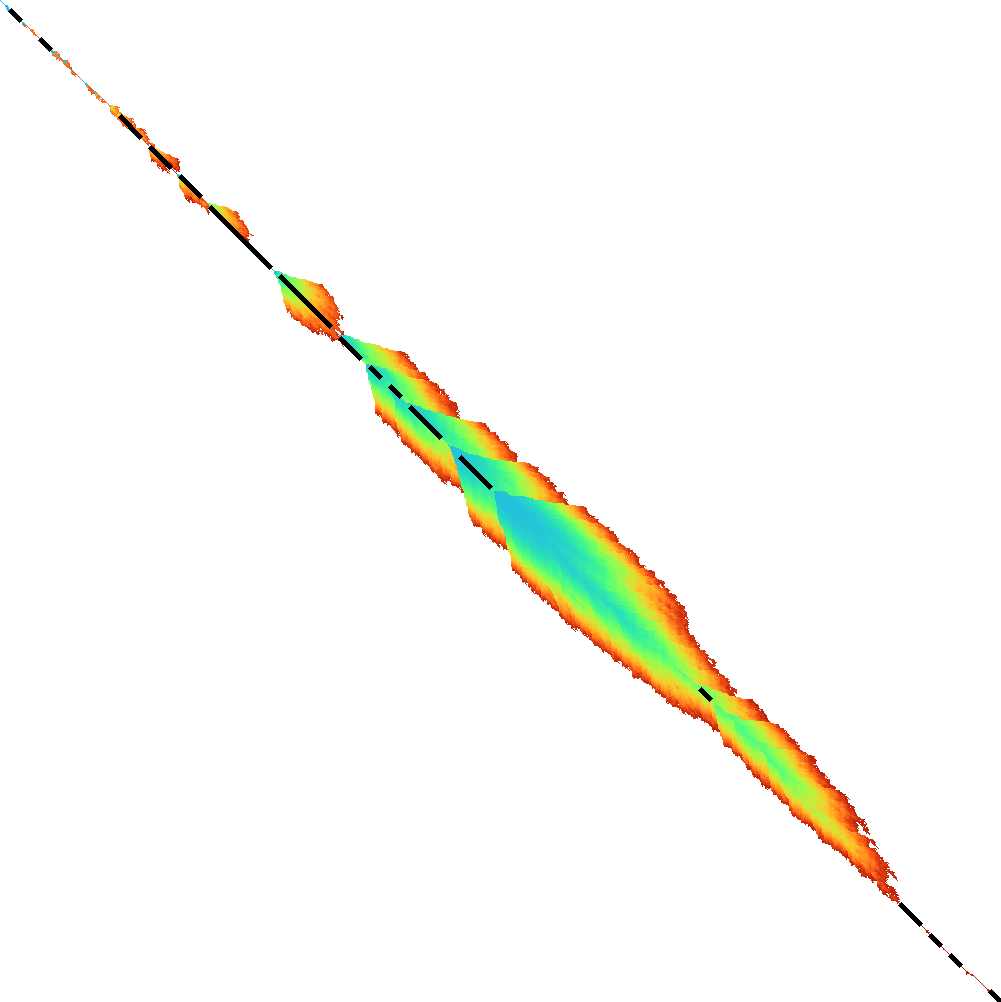
\includegraphics[height=0.31\linewidth]{imgs/fig8/high-error-rate.png}\label{GLOBALfig:high_error_rate}}
  %\hfill
  \subfloat[Long indel]
    {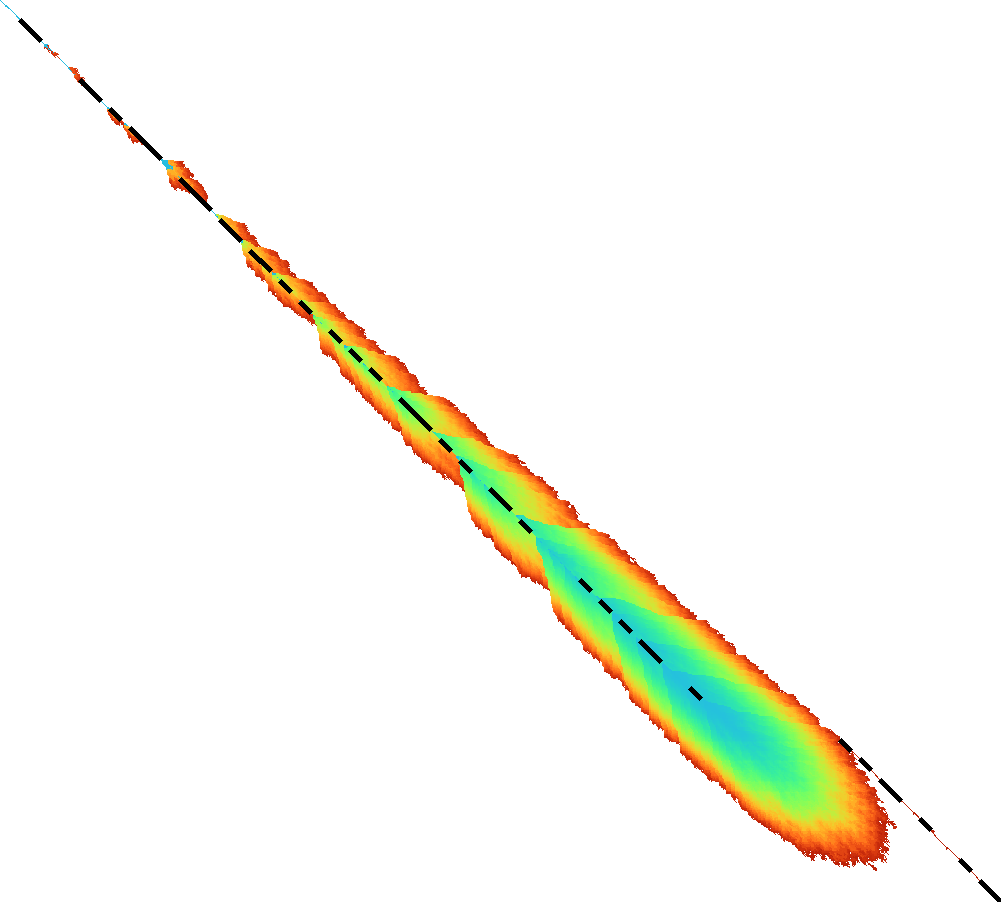
\includegraphics[height=0.31\linewidth]{imgs/fig8/deletion.png}\label{GLOBALfig:deletion}}
  %\hfill
  \subfloat[Short repeats]
    {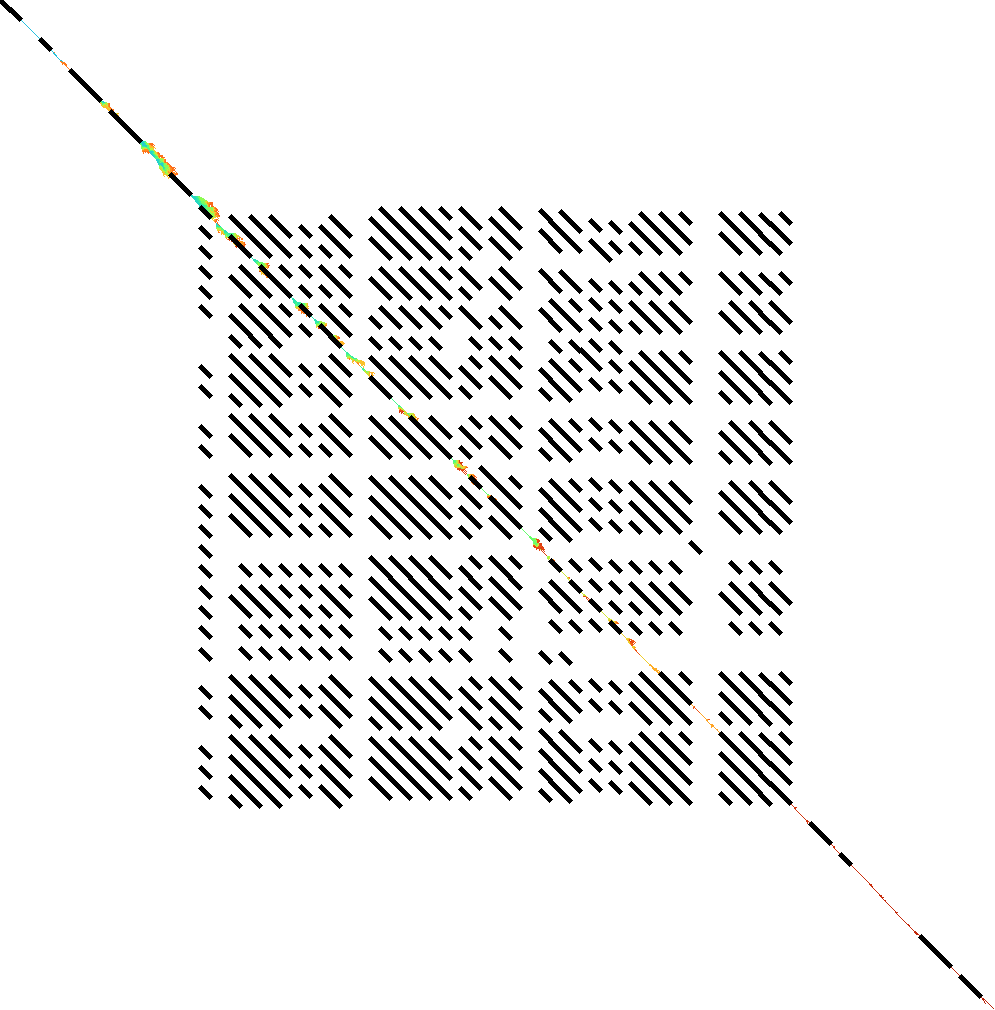
\includegraphics[height=0.31\linewidth]{imgs/fig8/repeats.png}\label{GLOBALfig:repeats}}
  \caption[Expanded states for various complex cases]{Expanded states by \CSH
  ($r{=}2$, $k{=}10$) in complex cases. The aligned pairs of \textbf{synthetic
  sequences} ($n{=}1000$) have $8\%$ uniformly random errors and contain (a) a
  region of length $200$ with larger error rate ($e{=}50\%$) than the heuristic
  can efficiently account for, (b) a deletion of length $100$, and (c) $60$
  mutated copies of a pattern of length $10$. Seed matches are shown in black
  and occur on the best paths and in the repeated region. The order of expansion
  is shown by the color gradient from blue to red.}
  \label{GLOBALfig:limitations}
\end{figure}

Our algorithm finds optimal alignments very efficiently when both the sequence
and the errors are uniformly random and the error rate is
limited~(\cref{GLOBALsec:evals}). Nevertheless, since the alignment problem is
fundamentally unsolvable in strictly subquadratic time~\citep{backurs2015edit},
there are sequences which cannot be aligned fast. We give three cases
(\cref{GLOBALfig:limitations}) for which the performance of our approach
degrades (possibly up to quadratic).

\begin{enumerate}
  \item \emph{High error rate.}
        When the error rate becomes too high (larger
        than $r/k$), seeds can not increase the heuristic enough
        penalize all errors. Each unpenalized error increases $f$ and needs more
        states to be searched, similar to \dijkstra.
        This can be mitigated by using shorter seeds and/or inexact matches, at
        the cost of introducing more matches.
  \item \emph{Long indel.}
        If there is a long insertion or deletion, the
        search has to accumulate the high cost for the long indel.
        Our heuristics do not account for long indels, and hence the search
        needs to expand states until the end of the gap is reached. Again, this
        causes a big increase of $f$ and a search similar to \dijkstra.
        This may be improved in future work by introducing a \emph{gap-cost} term to the \csh
        that penalizes gaps between consecutive matches in a chain.
  \item \emph{Short repeats.}
        When a short pattern repeats many times, this can result in a quadratic
        number of matches. This makes the corresponding seeds ineffective for
        the \sh, and slows down the computation and pruning of the \csh.
        This can be partially mitigated by increasing the seed length and/or
        exact matches, at the cost of reducing the potential of the heuristic.
        Alternatively, seeds with too many matches could be completely ignored.
\end{enumerate}
